\documentclass[11pt]{report}

\special{papersize=8.5in,11in}

\topmargin -0.5in \oddsidemargin 0.00in \evensidemargin 0.00in
\textwidth 6.75in \textheight 9.0in \headheight 0.25in \headsep
0.25in \footskip 0.5in \hoffset 0in \marginparpush 0.0in
\marginparwidth 0.0in \marginparsep 0.2in

\setcounter{page}{1}

\newcommand{\D}{\displaystyle}\newcommand{\T}{\textstyle}
\newcommand{\e}{{\mathrm{exp}}}
\newcommand{\dd}{{\mathrm d}}
\newcommand{\comment}[1]{}
\newcommand{\mb}{\mathbf}
\reversemarginpar

\usepackage[final]{graphicx}
\usepackage{fancyhdr}
%\graphicspath{{Papers/}}
\usepackage{amsthm,amssymb,amsmath}
\usepackage{cite}
\usepackage{geometry}
\usepackage{amsmath}
\usepackage{booktabs}
%\usepackage[top=2.5cm, bottom=2.5cm, right=3.5cm, left=3.5cm]{geometry}
\geometry{a4paper,scale=0.8}
\setcounter{secnumdepth}{4}

\title{Research Progress Report}

\author{Botao Zhu}

\begin{document}
	
	\maketitle
	
	\lhead{\sf Research Progress Report} \chead{} \rhead{\sf Botao Zhu}
	\lfoot{CTRG, University of Saskatchewan} \cfoot{} \rfoot{Page \thepage}
	\renewcommand{\footrulewidth}{1.0pt}
	\renewcommand{\headrulewidth}{2.0pt}
	\renewcommand{\arraystretch}{1.3}
	\pagestyle{fancy}
	
	\renewcommand{\thesection}{\arabic{section}}
	
	\section{Reading and Research Activities}
	
	\subsection{Summary}
	[1] proposed a deep learning based routing table construction method for a GPU-accelerated SDR. They adopted supervised Deep Belief Architectures(DBA) to compute the subsequent nodes with the traffic patterns of the edge routers as the input. And then, they presented unique characterizations of inputs and outputs based on the traffic patterns at the edge routers. They demonstrated how the trained DBA can predict the nodes, the benefits of the deep learning based routing strategy in terms of lower signaling overhead as well as fast convergence and effectiveness of proposed deep learning based solution compared to a benchmark routing method through both analysis and extensive. \\
	
	[2] aims to solve the following problems: (1) mitigate the traffic overhead imposed on BSs in disaster situations, (2) extend BS coverage through collaboration with wireless ad-hoc nextworks, (3) establish the maximum number of communication connections in situations in which network resources are insufficient and communication links are unstable. In this paper, the node degree of wireless communication is classified by deep learning for disaster situations and virtual routes are set according to the predetermined node by employing the Viterbi algorithm.
	
	\subsection{Deep Learning Based Routing Strategy}
	\subsubsection{Input and Output Design}
    The traffic pattern is served as the input to the deep learning structure and processed for routing path decision as the output. The traffic pattern at each router can be defined as the number of inbound packets of the router during each time interval,such as $\beta\bigtriangleup$t. Therefore, by assuming that a network comprises of N routers, we can use a matrix of $\beta$ rows and N columns to represent the traffic patterns of all routers. The simulation results demonstrate that it is accurate enough to set the value of $\beta$ to 1. The output layer can be designed to give the next node similar to the distributed routing strategy because of its lower complexity and higher tolerance. In the vector, only a single element has the value of 1, the order of which represents the next node.So, we can use two N dimensional vectors to represent the input and output.
	
	\subsubsection{Deep Learning Structure Design}
	The authors choose the DBA as the deep learning structures as shown in Figure 1.
	\begin{figure}[h!]
		\centering
		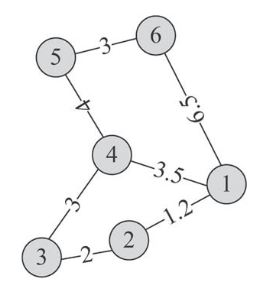
\includegraphics[width=0.5\linewidth]{figure1.png}
		\caption{Considered L-layer DBA}
		\label{fig-label}
	\end{figure}
	
	DBA can be also seen as a stack of $\left(L-2\right)$ Restricted Boltzmann Machines(RBM) and a logistic regression layer as the top layer. The structure of RBM consists of two layers, the visible layer, $\mb{v}$, and the hidden layer,$\mb{h}$, shown in Figure 2.
	\begin{figure}[h!]
		\centering
		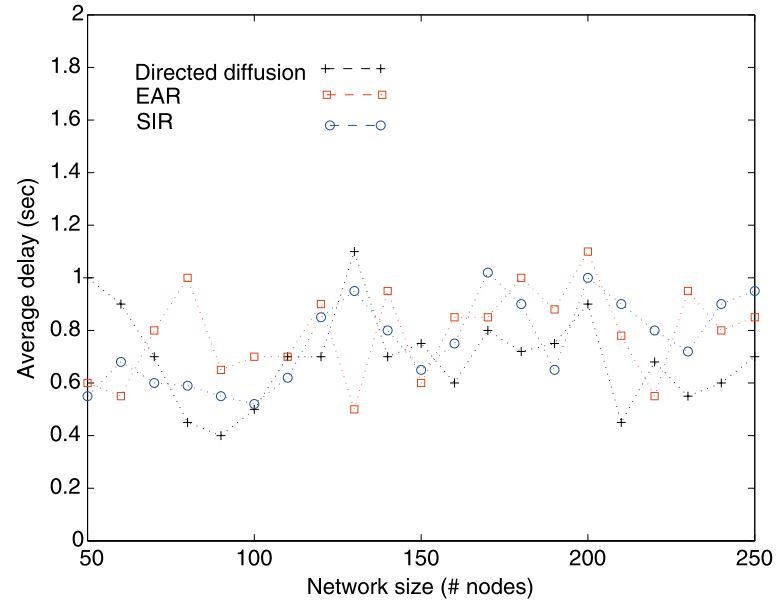
\includegraphics[width=0.5\linewidth]{figure2.png}
		\caption{RBM}
		\label{fig-label}
	\end{figure}
	While training an RBM, sets of unlabeled data are given to the visible layer, and the value of the weights and biases are repeatedly adjusted until the hidden layer can reconstruct the visible layer. To mathematically model the training process, they use a log-likelihood function of the visible layer given as follows.
	\begin{equation}
	l\left(\theta,a\right)=\sum_{t=1}^{m}\log{p\left(v^t\right)}
	\end{equation}
	where $\theta$ denotes the vector consisting of all the values of the weights and biases of the hidden layer.\\
	%Since RBM is a particular form of log-linear Markov Random Field, the energy function, $\E\left(v,h\right)$, and the joint probability function, $p\left(v,h\right)$, are defined as follows:\\
	\begin{eqnarray}
	E\left(v,h\right) &=& -\sum_{i}a_iv_i-\sum_{j}b_jh_j-\sum_{i}\sum_{j}h_jw_{ji}v_i\\
	p\left(v,h\right) &=& \frac{e^{-E\left(v,h\right)}}{Z}\\
	Z &=& \sum_{v}\sum_{h}e^{-E\left(v,h\right)}
	\end{eqnarray}
	where $v_i$ and $h_j$ are the unit $i$ in the visible layer and the unit $j$ in the hidden layer respectively. $Z$ represents the normalizing constant partition function. Also, the relationship between $p\left(v\right)$ and $p\left(v,h\right)$ can be expressed as follows:\\
	\begin{equation}
	p\left(v\right)=\sum_{h}\left(v,h\right)
	\end{equation}
	However, the complexity of the calculation is extremely high. To solve this problem, they use the Gibbs Sampling method to sample the values of $v$ and $h$ to approximate the real values since the conditional distribution probability of one layer can be calculated. As each unit is independent on the other units in the same layer, when one layers is fixed, the conditional distribution probability of the other layer can be calculated as follows:
	\begin{eqnarray}
	p\left(v|h;\theta,a\right) &=& \prod_{i}p\left(v_i|h;\theta,a\right)\\
	p\left(h|v;\theta,a\right) &=& \prod_{j}p\left(h_j|v;\theta,a\right)
	\end{eqnarray}
	Since input units are continuous, they use Gaussian probability distribution to model the traffic patterns. Equations$\left(2\right)$ and $\left(6\right)$ should be revised as follows:
	\begin{eqnarray}
	E\left(v,h\right) &=& -\sum_{i}\frac{\left(v_i-a_i\right)^2}{2{\delta_i}^2}-\sum_{j}b_jh_j-\sum_{i}\sum_{j}\frac{v_i}{\delta_i}h_jw_{ji}\\
	p\left(v_i|h;\theta,a\right) &=& N\left(a_i+\delta_i\sum_{j}h_jw_{ji},{\delta_i}^2\right)	
	\end{eqnarray}
	where $\delta_i$ is the value of the variance for the unit $v_i$. 
	However, in Figure 3, we can see that the visible layer of $RBM_{L-2}$ consists of not only $RBM_{L-3}$'s hidden layer but also the output layer of the DBA, $y$. Its hidden layer is the top hidden layer of the DBA and energy function is expressed as follows.
	\begin{figure}[h!]
		\centering
		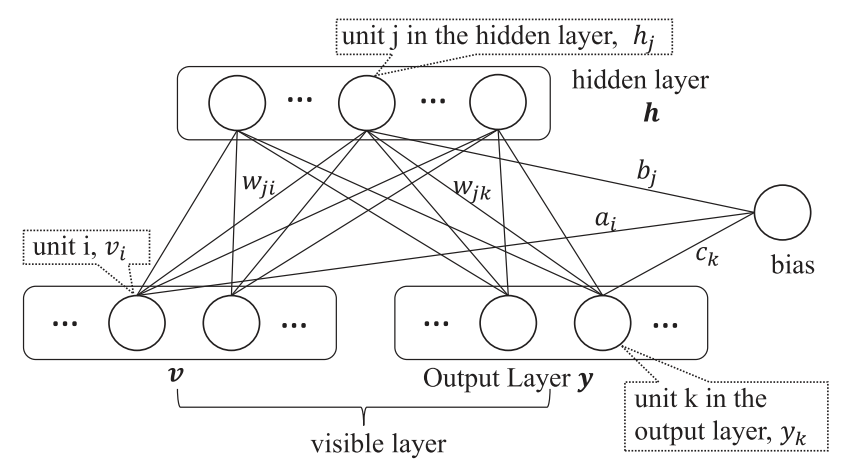
\includegraphics[width=0.5\linewidth]{figure3.png}
		\caption{Last RBM}
		\label{fig-label}
	\end{figure}
	\begin{equation}
	E\left(v,h,y\right) = -\sum_{i}a_iv_i-\sum_{j}b_jh_j-\sum{k}c_ky_k-\sum_{i}\sum_{j}h_jw_{ji}v_i-\sum_{j}\sum_{k}h_jw_jky_k
	\end{equation}
	where $y$ represents the vector in the output layer. $c_k$ is the bias of the unit $y_k$. $w_{jk}$ represents the weight of the link connecting the units $h_j$ and $y_k$. The conditional distribution of the concatenated vector consisting of $v$ and $y$ is,
	\begin{eqnarray}
	p\left(v,y|h;\theta,a\right) &=& p\left(v|h;\theta,a\right)p\left(y|h;\theta,a\right)\\
	&=&\prod_{i}p\left(v_i|h;\theta,a\right)\prod_{k}p\left(y_k|h;\theta,a\right)
	\end{eqnarray}
	The purpose of supervised training is to minimize the difference between the output of the DBA and the labeled output $y$. They use the cross-entropy cost function to measure their difference given as bellow.\\
	They use the cross-entropy cost function to measure the difference between the output of the DBA, denoted by $h_\theta\left(x\right)$, and the labeled output $y$.
	\begin{equation}
	C\left(\theta\right)=-\frac{1}{m}\sum_{t=1}^{m}\left(y^t\log\left(h_\theta\left(x^t\right)\right)+\left(1-y^t\right)\log\left(1-h_\theta\left(x^t\right)\right)\right)+\frac{\lambda}{2}\sum_{l=2}^{L}\sum_{j=1}^{n_l}\sum_{i=1}^{n_{l-1}}\left({w_{ji}}^l\right)^2
	\end{equation}
	$\left(x^t,y^t\right)$ is the $t$th training data. $h_\theta\left(x^t\right)$ denotes the output of the DBA. $C\left(\theta\right)$ consists of two parts: the difference between the output of DBA and the labeled output, keeping the training process from overfitting. Using the gradient descent to update $\theta$ to minimize the value of $C\left(\theta\right)$. $\eta_{bp}$ is the learning rate in the back-propagation process.
	\begin{equation}
	\theta:=\theta-\eta_{bp}\frac{\partial C\left(\theta\right)}{\partial\theta}
	\end{equation}
	
	\subsubsection{The Procedures of the Proposed Deep Learning Based Routing Strategy}
	\paragraph{Initialization Phase}
	The goal of the initialization phase is to obtain the labeled data which consist of the input vector and the corresponding output vector. They approach a number of available data set sources, such as the center for applied internet data analysis, and extract the traffic information and relevant routing paths.
	\paragraph{Training Phase}
    The training phase consists of two steps: the loop of the Greedy Layer-Wise training to train each RBM and the following backpropagation process to fine-tune the weights of links between the layer. Let $\mathnormal{N}$ and $\mathnormal{I}$ denote the total number of routers and the number of inner routers. So,every edge router needs to train $\left(\mathnormal{N} - \mathnormal{I} - 1\right)$ DBAs while each inner router needs to train $\left(\mathnormal{N} - \mathnormal{I}\right)$ DBAs. Then, every edge router needs to send its $\theta$ of $\left(\mathnormal{N} - \mathnormal{I} -1\right)$ to other $\left(\mathnormal{N} - \mathnormal{I} -1\right)$ edge routers. Every inner router needs to send its $\theta$ of $\left(\mathnormal{N} - \mathnormal{I}\right)$ DBAs to all the edge routers. Therefore, each edge router obtains $\theta$ of all the DBAs of all the routers in the network, and the number of sets of $\theta$ is $\left(\mathnormal{N} - \mathnormal{I}\right)\left(\mathnormal{N} - 1\right)$.\\
     
	\begin{tabular}{lc}
		\toprule
		\textbf{Algorithm 1}. Supervised Train DBA\\
		\hline
		\textbf{Input:} $\left(x,y\right)=\{\left(x^t,y^t\right)|t=1,...,m\}, \eta_{CD}, \eta_{bp},L, n=\left(n_1,...,n_L\right)$\\
		\textbf{Output: $\theta$}\\
		1: \textbf{for} $i=1,...,L-2$ \textbf{do}\\
		2: \quad TrainRBM $\left(u^i,\eta_{CD},n_i,n_{i+1}\right)$\\
		3: \textbf{end for}\\
		4: Fine-tuneDBA$\left(\left(x,y\right),\theta,\eta_{bp}\right)$\\
		5: \textbf{return} $\theta$\\
		\hline
	\end{tabular}
	\paragraph{Running Phase}
	Every edge router can utilize the next node information to construct the whole paths from itself to all the other edge routers. They use an array of $\mathnormal{N}$ elements, $\mathcal{TP}\left[\mathnormal{N}\right]$, to save the numbers of inbound packets of $\mathnormal{N}$ routers in the network to represent the traffic patterns, and $\theta\left[\mathnormal{N} - \mathnormal{I}\right]\left[\mathnormal{N} - 1\right]$ to save the parameters of all the DBAs in the network. Another array $\mathcal{ER}\left[\mathnormal{N} - \mathnormal{I}\right]$ is used to save the sequence numbers of the edge routers in the network since they are not continuous. Each edge router can obtain the outputs of DBAs to construct the paths to $\left(\mathnormal{N} - \mathnormal{I} - 1\right)$ edge routers. And then using a matrix, $\mathcal{NR}\left[\mathnormal{N}\right]\left[\mathnormal{N} - \mathnormal{I} - 1\right]$, to save the results of these DBAs that can be used to build the whole paths to all the other edge routers. Figure 4 is the routing model and Table 1 is an example of the routing table.\\

	\begin{table}[!h]
		\centering
		\caption{Routing table of $R_3$}
		\begin{tabular}{lc}
			\toprule
			Dest& Path\\
			\hline
			$R_1$& $R_3 \to R_2 \to R_1$\\
			$R_2$& $R_3 \to R_2$\\
			\dots& \dots\\
			$R_{16}$& $R_3 \to R_7 \to R_{11} \to R_{15} \to R_{16}$\\
			\hline
		\end{tabular}
	\end{table}

	\begin{figure}[h!]
		\centering
		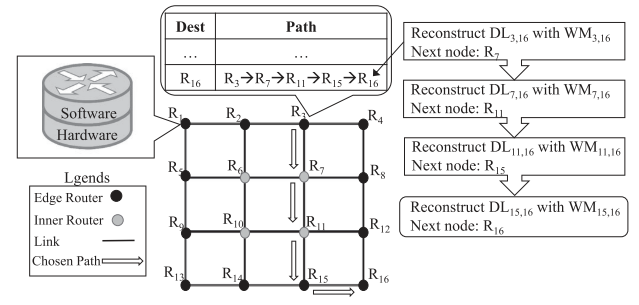
\includegraphics[width=0.5\linewidth]{figure4.png}
		\caption{Routing model}
		\label{fig-label}
	\end{figure}

	\subsection{Classification of node degree based on deep learning routing method applied for virtual route assignment}
	
	\subsubsection{Input and Output Design}
	
	\section{Objectives for the Next 2 Weeks}
	
	
	\section{Advisor's Comments}
	

	I'm very happy.cite \cite{IEEEexample:IEEEwebsite}
	\bibliographystyle{IEEEtran}
	
	\bibliography{IEEEexample}
	
\end{document}